\documentclass[14pt]{extreport}
\usepackage{gost}
%\usepackage{hyperref}
%\usepackage{makecell}
\usepackage{ragged2e}
%\usepackage{graphicx}%Вставка картинок правильная
%\usepackage{float}%"Плавающие" картинки
%\usepackage{wrapfig}%Обтекание фигур (таблиц, картинок и прочего)
%\justifying
\usepackage{listings}
\makeatletter
\@addtoreset{figure}{part}% Reset figure numbering at every part
\makeatother
\renewcommand{\thefigure}{\arabic{figure}}% Figure number is part.figure
\renewcommand{\thetable}{\arabic{table}}

%Тут можно вставить дополнительные пакеты

\begin{document}
    \pagestyle{empty} %  выключаем нумерацию
    
\includepdf[pages=-,pagecommand={}]{title_page.pdf}

    \pagestyle{plain} % включаем нумерацию
    \tableofcontents
    \intro В данной работе исследуется статистический анализ выборки из 20 чисел. Целью является определение вариационного ряда, выявление экстремальных значений и размаха, оценка математического ожидания и среднеквадратического отклонения, а также построение графических представлений, включая эмпирическую функцию распределения, гистограмму и полигон приведенных частот группированной выборки. При этом используется программная реализация на выбранном языке программирования.

    \chapter{Разработка программы на языке Python}
        \section{Введение}
        В результате выполнения работы была разработана программа на языке программирования Python, предназначенная для анализа статистических характеристик выборки из 20 чисел. Программа реализует расчет вариационного ряда, определение экстремальных значений и размаха, а также проводит оценку математического ожидания и среднеквадратического отклонения.

        Дополнительно, программа создает эмпирическую функцию распределения и строит ее график, предоставляя визуальное представление распределения данных. Кроме того, реализована возможность построения гистограммы и полигона приведенных частот группированной выборки для более наглядного анализа.
        \newpage
        \section{Листинг кода}
        \begin{figure}[!h]
            \centering
            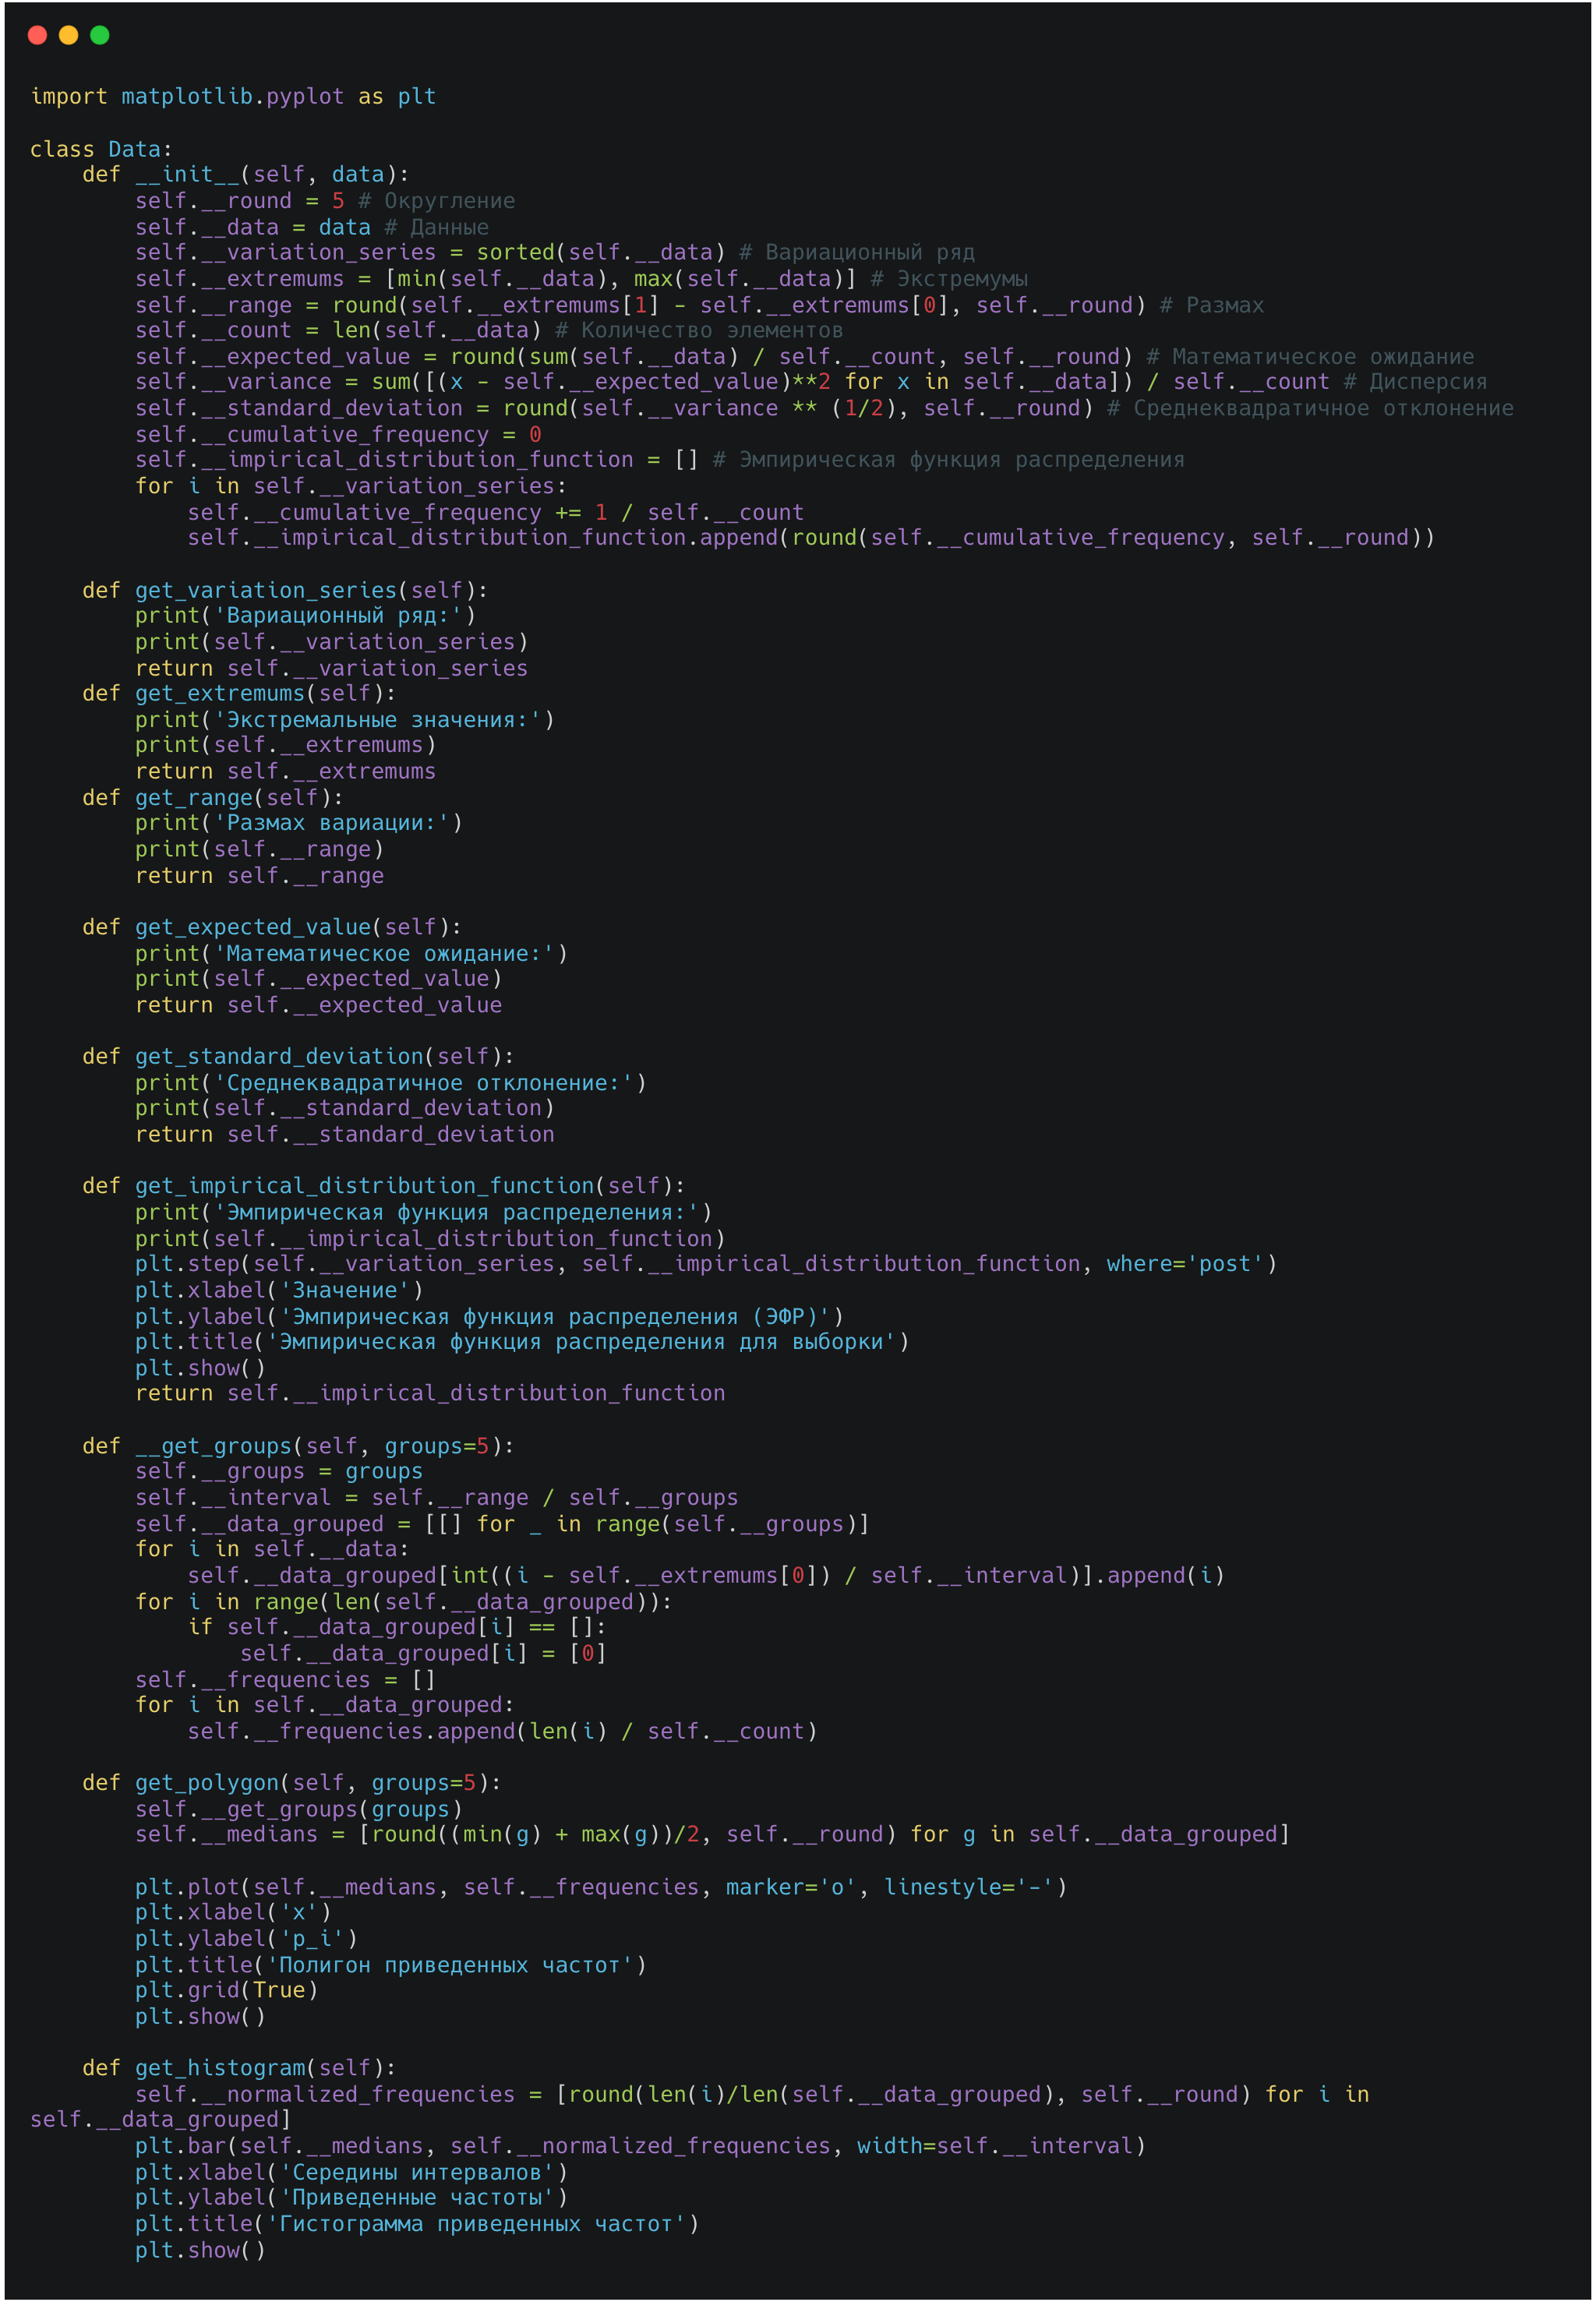
\includegraphics[width=0.87\linewidth]{code.png}
            \caption{Листинг кода}
        \end{figure}

        \section{Результаты программы}
            Программа успешно провела анализ предоставленной выборки, предоставив необходимые статистические характеристики и графические представления, такие как вариационный ряд, экстремальные значения, размах, математическое ожидание, среднеквадратичное отклонение и эмпирическая функция распределения. Графики полигона приведенных частот и гистограммы позволяют визуально оценить распределение данных в выборке.
            \begin{figure}[!h]
                \centering
                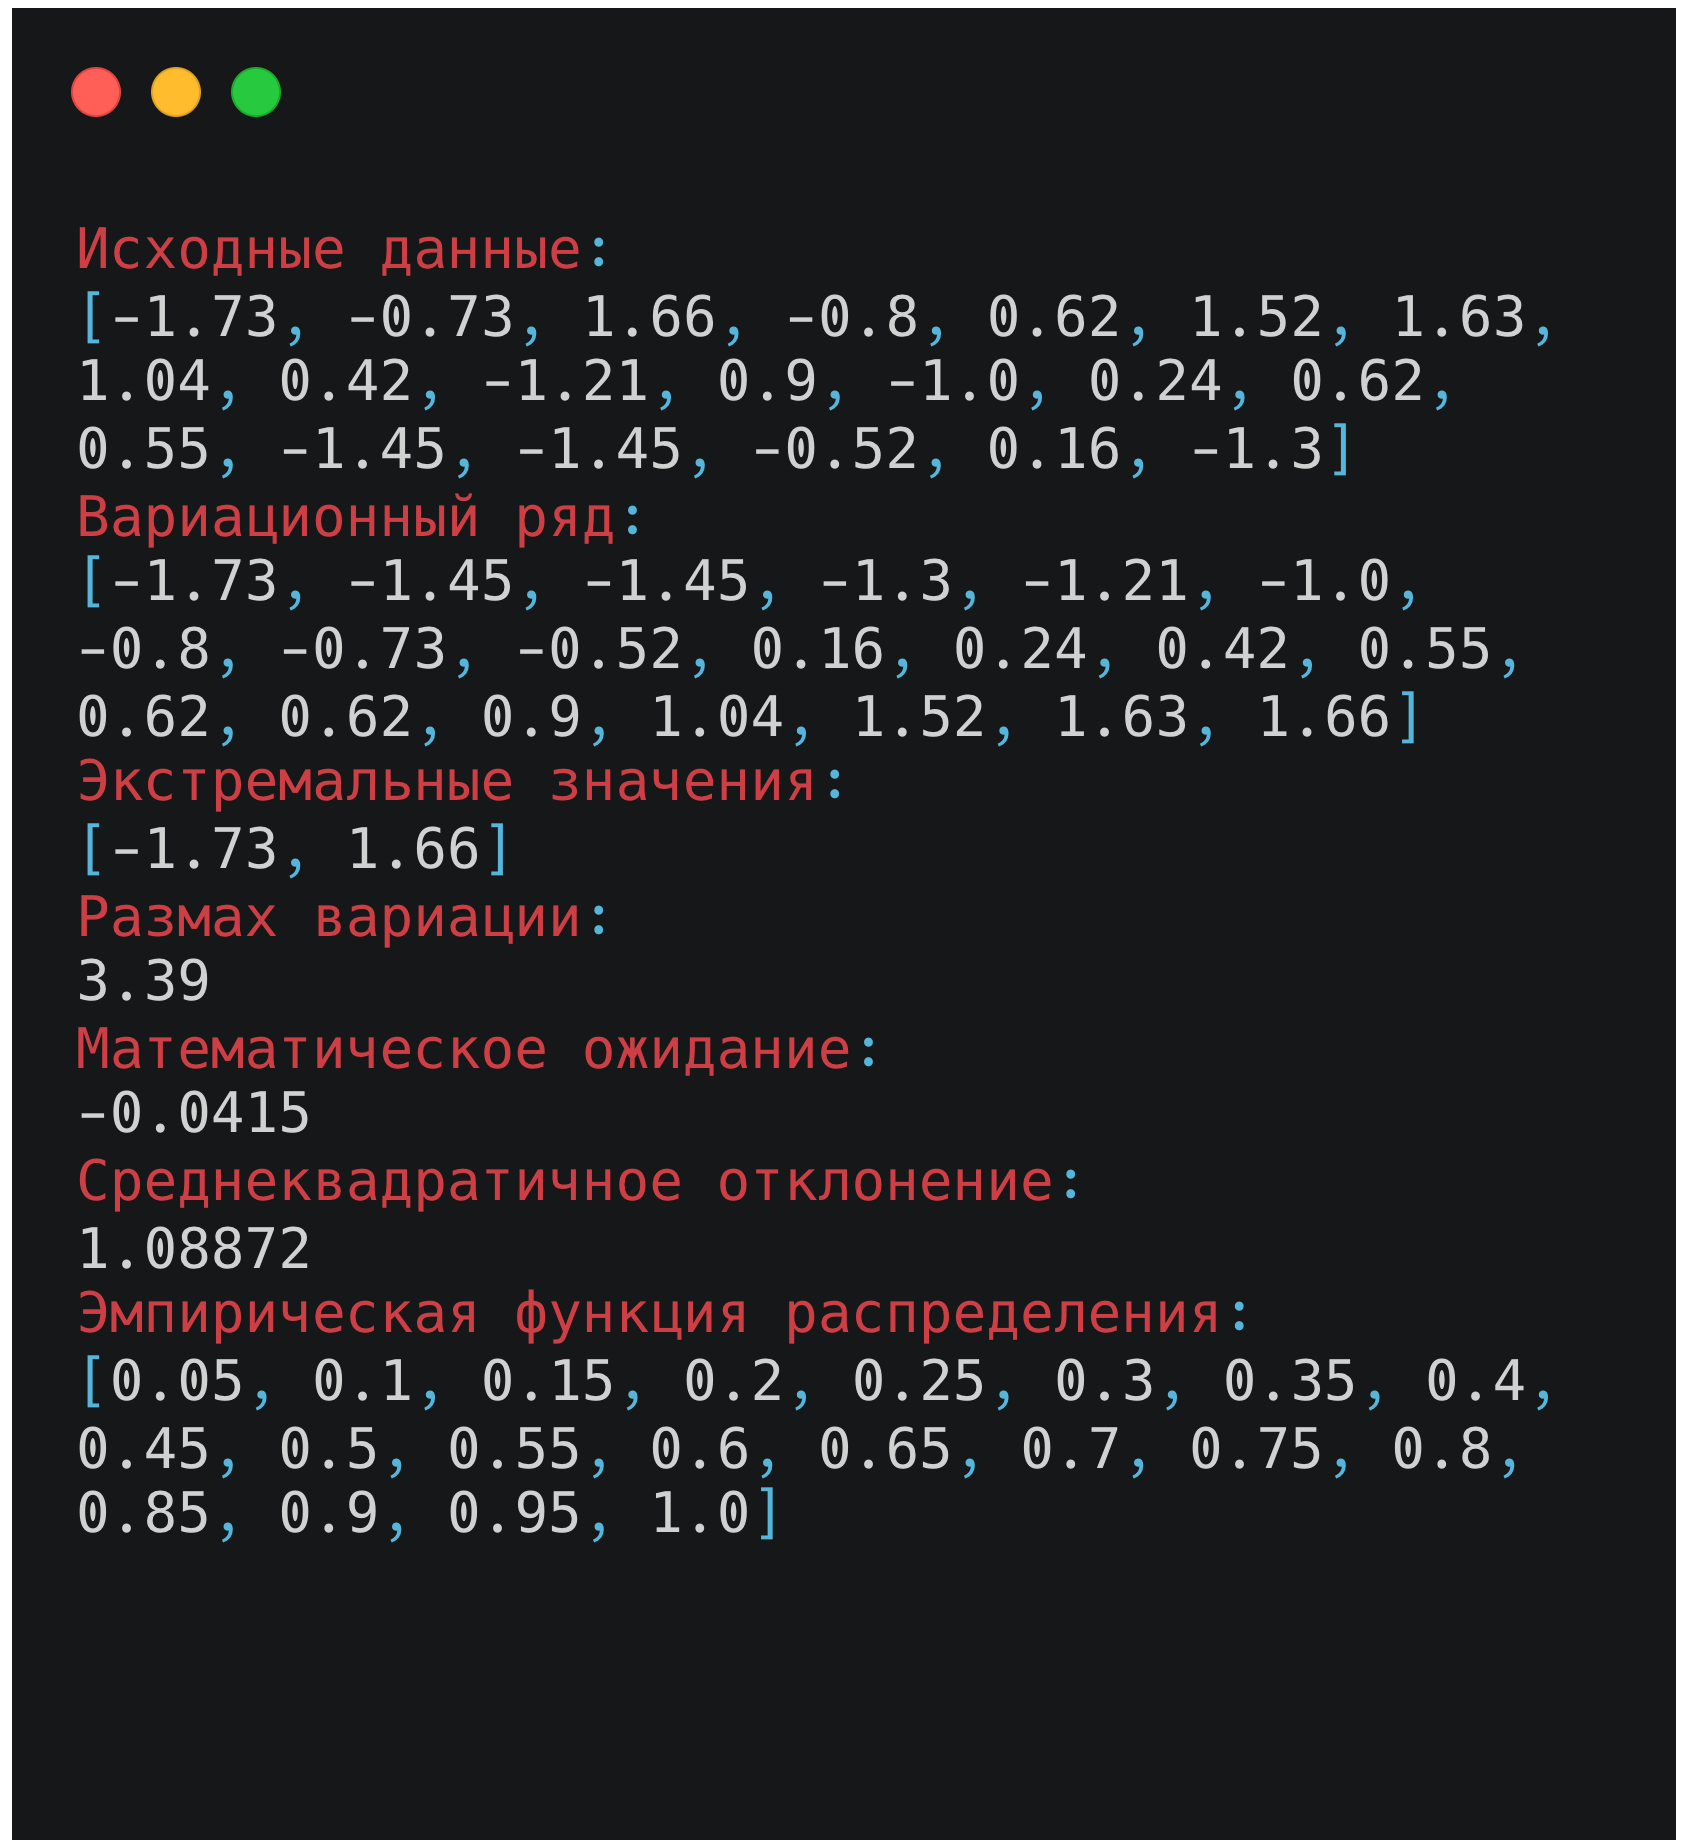
\includegraphics[width=0.5\linewidth]{result.png}
                \caption{Результат }
            \end{figure}

        \section{Графики}
            График представляет собой ступенчатую функцию, где по оси x отложены значения вариационного ряда, а по оси y - накопленные относительные частоты. Характеризует вероятность того, что случайная величина примет значение, не превосходящее заданное.
            \begin{figure}[!h]
                \centering
                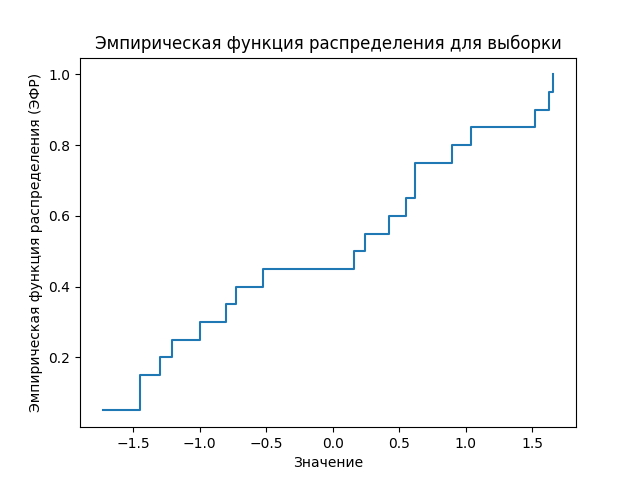
\includegraphics[width=0.3\linewidth]{graph1.png}
                \caption{График эмпирической функции распределения}
            \end{figure}

            График представляет собой линии, соединяющие середины интервалов группированной выборки. По оси x отложены значения медиан интервалов, а по оси y - приведенные частоты. Визуально отображает форму распределения и позволяет выявить особенности.
            \begin{figure}[h]
                \centering
                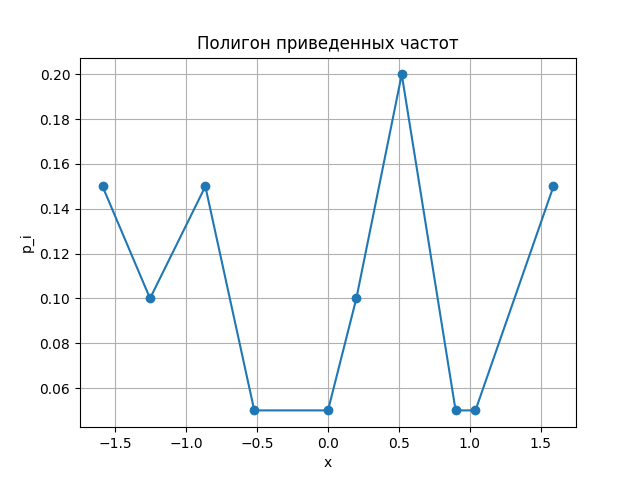
\includegraphics[width=0.3\linewidth]{graph2.png}
                \caption{Полигон приведенных частот }
            \end{figure}

            Гистограмма представляет собой столбцы, высота которых пропорциональна приведенным частотам группированной выборки. Ось x отражает середины интервалов, а ось y - приведенные частоты. Позволяет оценить форму и интенсивность распределения данных.
            \begin{figure}[h]
                \centering
                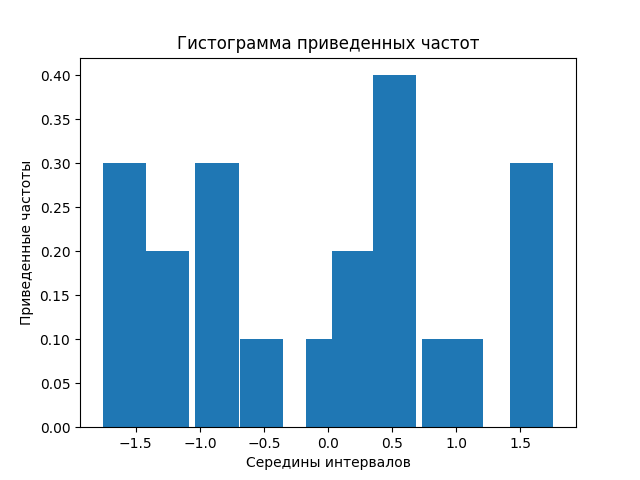
\includegraphics[width=0.3\linewidth]{graph3.png}
                \caption{Гистограмма приведенных частот }
            \end{figure}
    \conclusions В ходе анализа предоставленной выборки были успешно рассчитаны и визуализированы основные статистические характеристики. Вариационный ряд, экстремальные значения и размах, оценки математического ожидания и среднеквадратического отклонения, а также эмпирическая функция распределения были получены и представлены графически. Гистограмма и полигон приведенных частот дополнили обзор, позволяя визуально оценить структуру и распределение данных. Полученные результаты способствуют более глубокому пониманию характеристик выборки и её статистического поведения.






\end{document}